\section{Transfer Learning: Representing contacts}
\label{sec:InfoForPrediction}
\begin{figure}[t]
\centerline{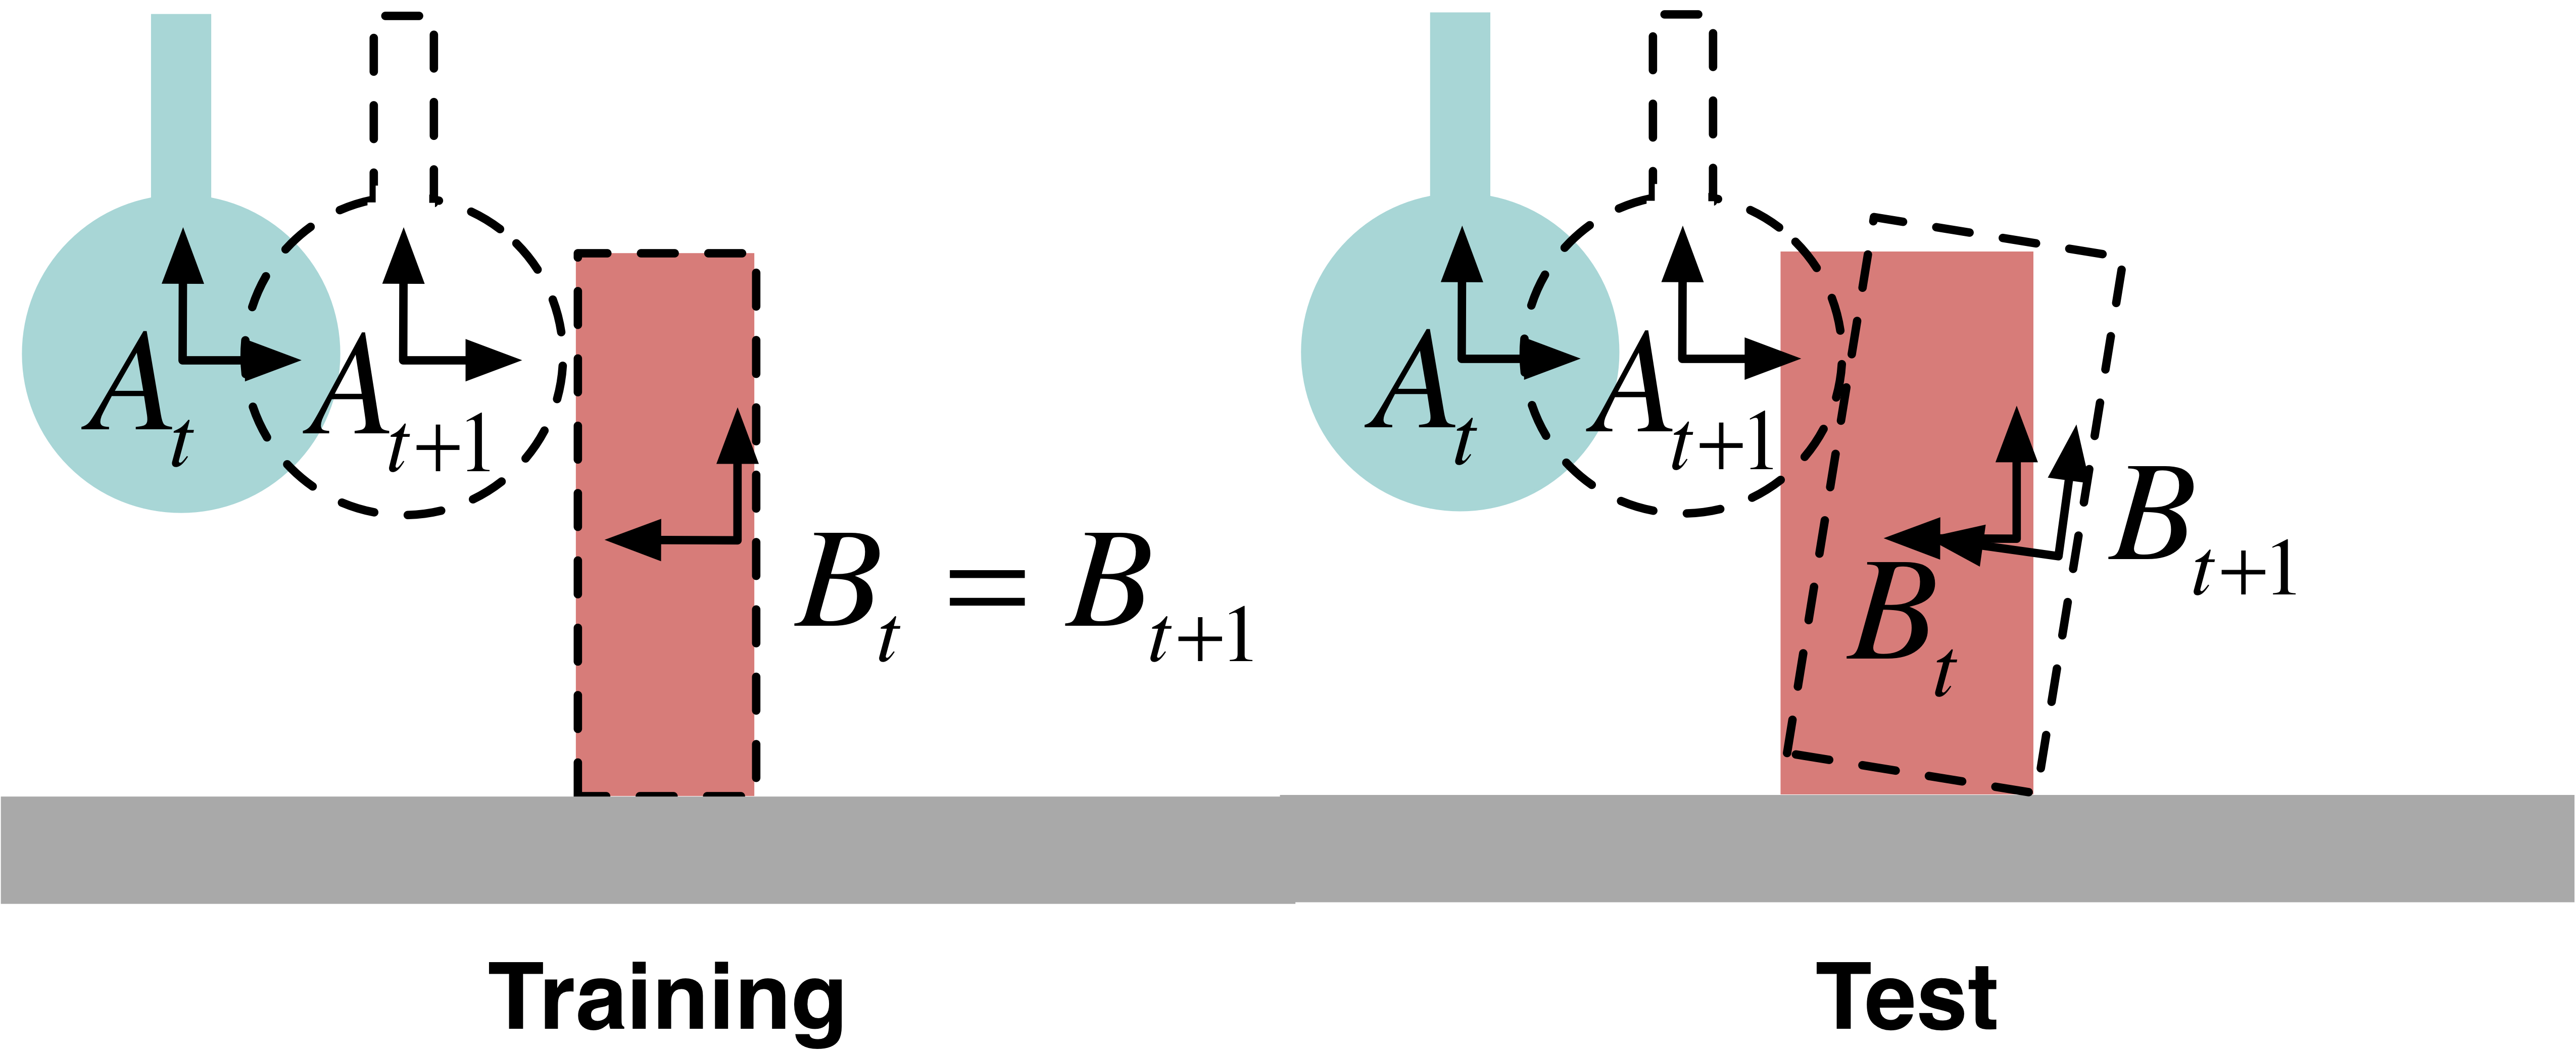
\includegraphics[width=\columnwidth]{shapes-colour}}
\caption[Shapes]{Two scenes (left and right),
each with an object on a tabletop. Only the shape of object $B$ differs between the scenes. Yet when finger A moves as shown by the dashed outline at time $t+1$, the resulting transformation of $B$ will be quite different.}
\label{fig:Learning.shapes}
\end{figure}
The input domains of $f$, $f_{qs}$, and $p_{qs}$ are insufficient to pose problems P2 (Action Transfer) or P3 (Shape Transfer). This is because they only capture the {\em global} relations between objects. To properly pose transfer learning the input domain must capture all the {\em local} contact relations between the object and its surroundings.  To see why, consider Figure~\ref{fig:Learning.shapes}. On the left is a training example. On the right is a test case, where the object is wider. Given the same placement of the frames on object and agent, and the same finger motion, the predicted behaviour using Equation~\eqref{eq:Learning.short} will be the same as for the training example. This is wrong. For the correct prediction to be transferred, additional information is needed on the contact between $A$ and $B$. This can be captured by attaching additional frames to $A$ and $B$ close to their point of contact (see Figure~\ref{fig:Learning.setup2}, centre panel).
\begin{figure*}[t]
\centerline{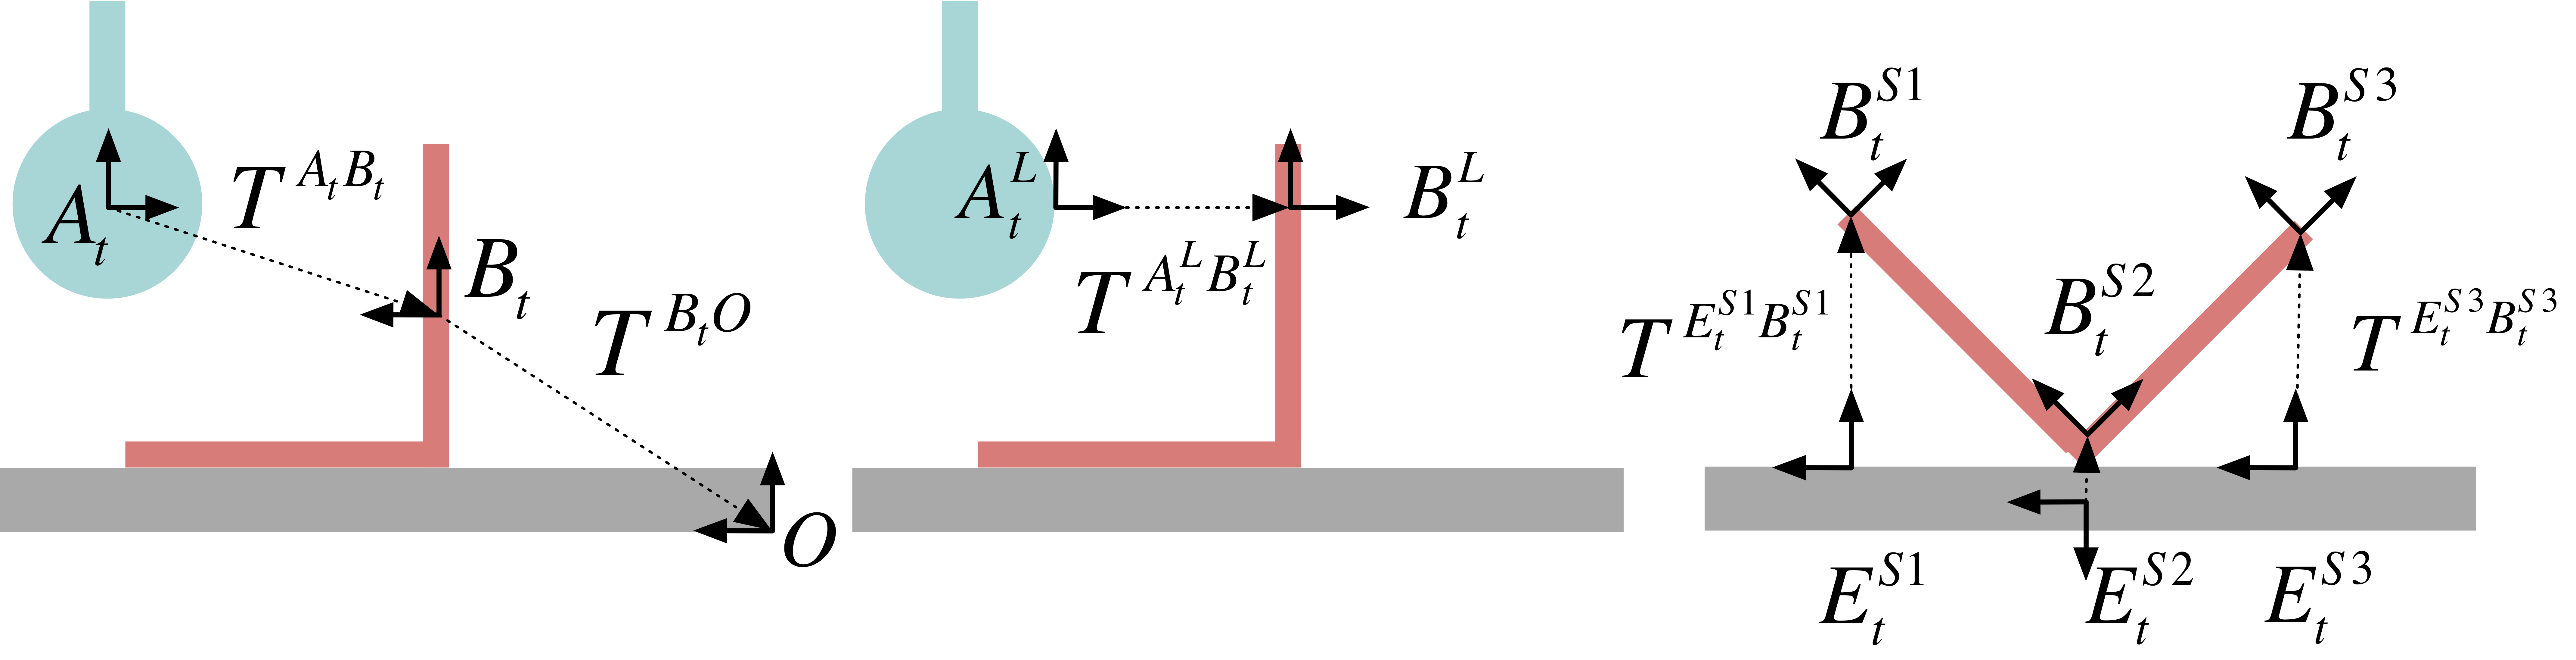
\includegraphics[width=\textwidth]{information}}
\caption{Three types of information useful in prediction problems. Left: (G - global) global frames of reference for the robot, object and the world. Centre: (A - agent) local frames of reference on the robot finger and the closest point on the object. Right (E - environment) local frames of reference on the object and the closest points on surfaces in the environment.}
\label{fig:Learning.setup2}
\end{figure*}
In general, an object has multiple contacts with the robot and the environment. Each of these contacts provides a kinematic constraint on the object's motion, and thus each one should be modelled. Rigid body simulators use just such contact information. 

We use a pair of local frames to encode each contact or near contact. Each pair encodes one transformation between part of the object $B$ and another body.  To distinguish these local frame pairs from what has gone before we henceforth refer to the main frame attached to a body (defined in Section~\ref{sec:Representations}) as that body's global frame. We define the local frame pairs as follows. Consider Figure~\ref{fig:Learning.setup2}  (left panel). We first define a pair of local frames capturing the finger-object contact as $A^{L}_{t}$ and $B^{L}_{t}$ (centre panel). These are spatially dynamic, i.e.\ at any time $t$ they are located at the points of closest proximity on the finger and object respectively.  We define the \textit{agent-object contact}
information as the transformations $T^{A^{L}_{t}, A^{L}_{t+1}}$ and $T^{A^{L}_t, B^{L}_t}$.

We also define local frame pairs to model object-environment contacts. One frame is attached to some point on the object ($B^{Sk}_t$), and one is attached to the nearest point in the environment $E^{Sk}_t$.  Thus the environment frame within each pair is spatially dynamic, changing its position as the object moves. If $N$ points on the object are chosen for modelling there will be $N$ pairs of local frames $B^{Sk}_t$ and $E^{Sk}_t$ to capture the object-environment contacts at time $t$, where ($k=1 \ldots N$) (Figure~\ref{fig:Learning.setup2} right panel). Using these frame pairs we then define the \textit{object-environment contact} information as the set of transformations $T^{E^{Sk}_t,B^{Sk}_t}$ for $k=1 \ldots N$. 

During training a single type of contact model is learned by pooling data from frames located at several points on the object. During transfer this single model is copied, creating several identical contact experts on the new object. An extension would be to condition a number of such contact models by the local shapes at the contacts, and this is an intended line of future work. We hypothesize that both data pooling and conditioning will be important elements in improving the transfer of predictions. Additionally, to obtain the results presented in this paper, the number and the locations of the frames $B^{Sk}_t$ on each different object were determined empirically.\footnote{This procedure could be automated.} Finally, we note that we have motivated these contact experts as enabling shape transfer, but they are equally applicable to action transfer. The top row of Figure~\ref{fig:ToyExample} shows a training and a test case for problem P2 (action transfer). The prediction for the test case requires encoding of the kinematic constraint imposed by the contact between the base of the L-shaped flap and the table. This constraint exists in the training push, but was not significant since the flap could rotate on its corner.

We can now consider the effects that different sets of information might have. A predictor possessed only
of global frames for each body we refer to as having global information (G). We add agent-object contact
information (G+A), and object-environment contact information (G+A+E). Now consider the possible predictions for the test case (Figure~\ref{fig:ToyExample} bottom row). A predictor using G will predict that the object will not move. A predictor using G+A has information from the training case that the object surface will move with the finger, so that the finger will not pass through it, but is also capable of predicting that the object rotates about the corner and into the table since it doesn't model the object-environment contact. A predictor using G+A+E will have information about the effect of the contact between the base of the flap and the table and so should avoid predicting a rotation into the table.
\begin{figure}[b]
\centerline{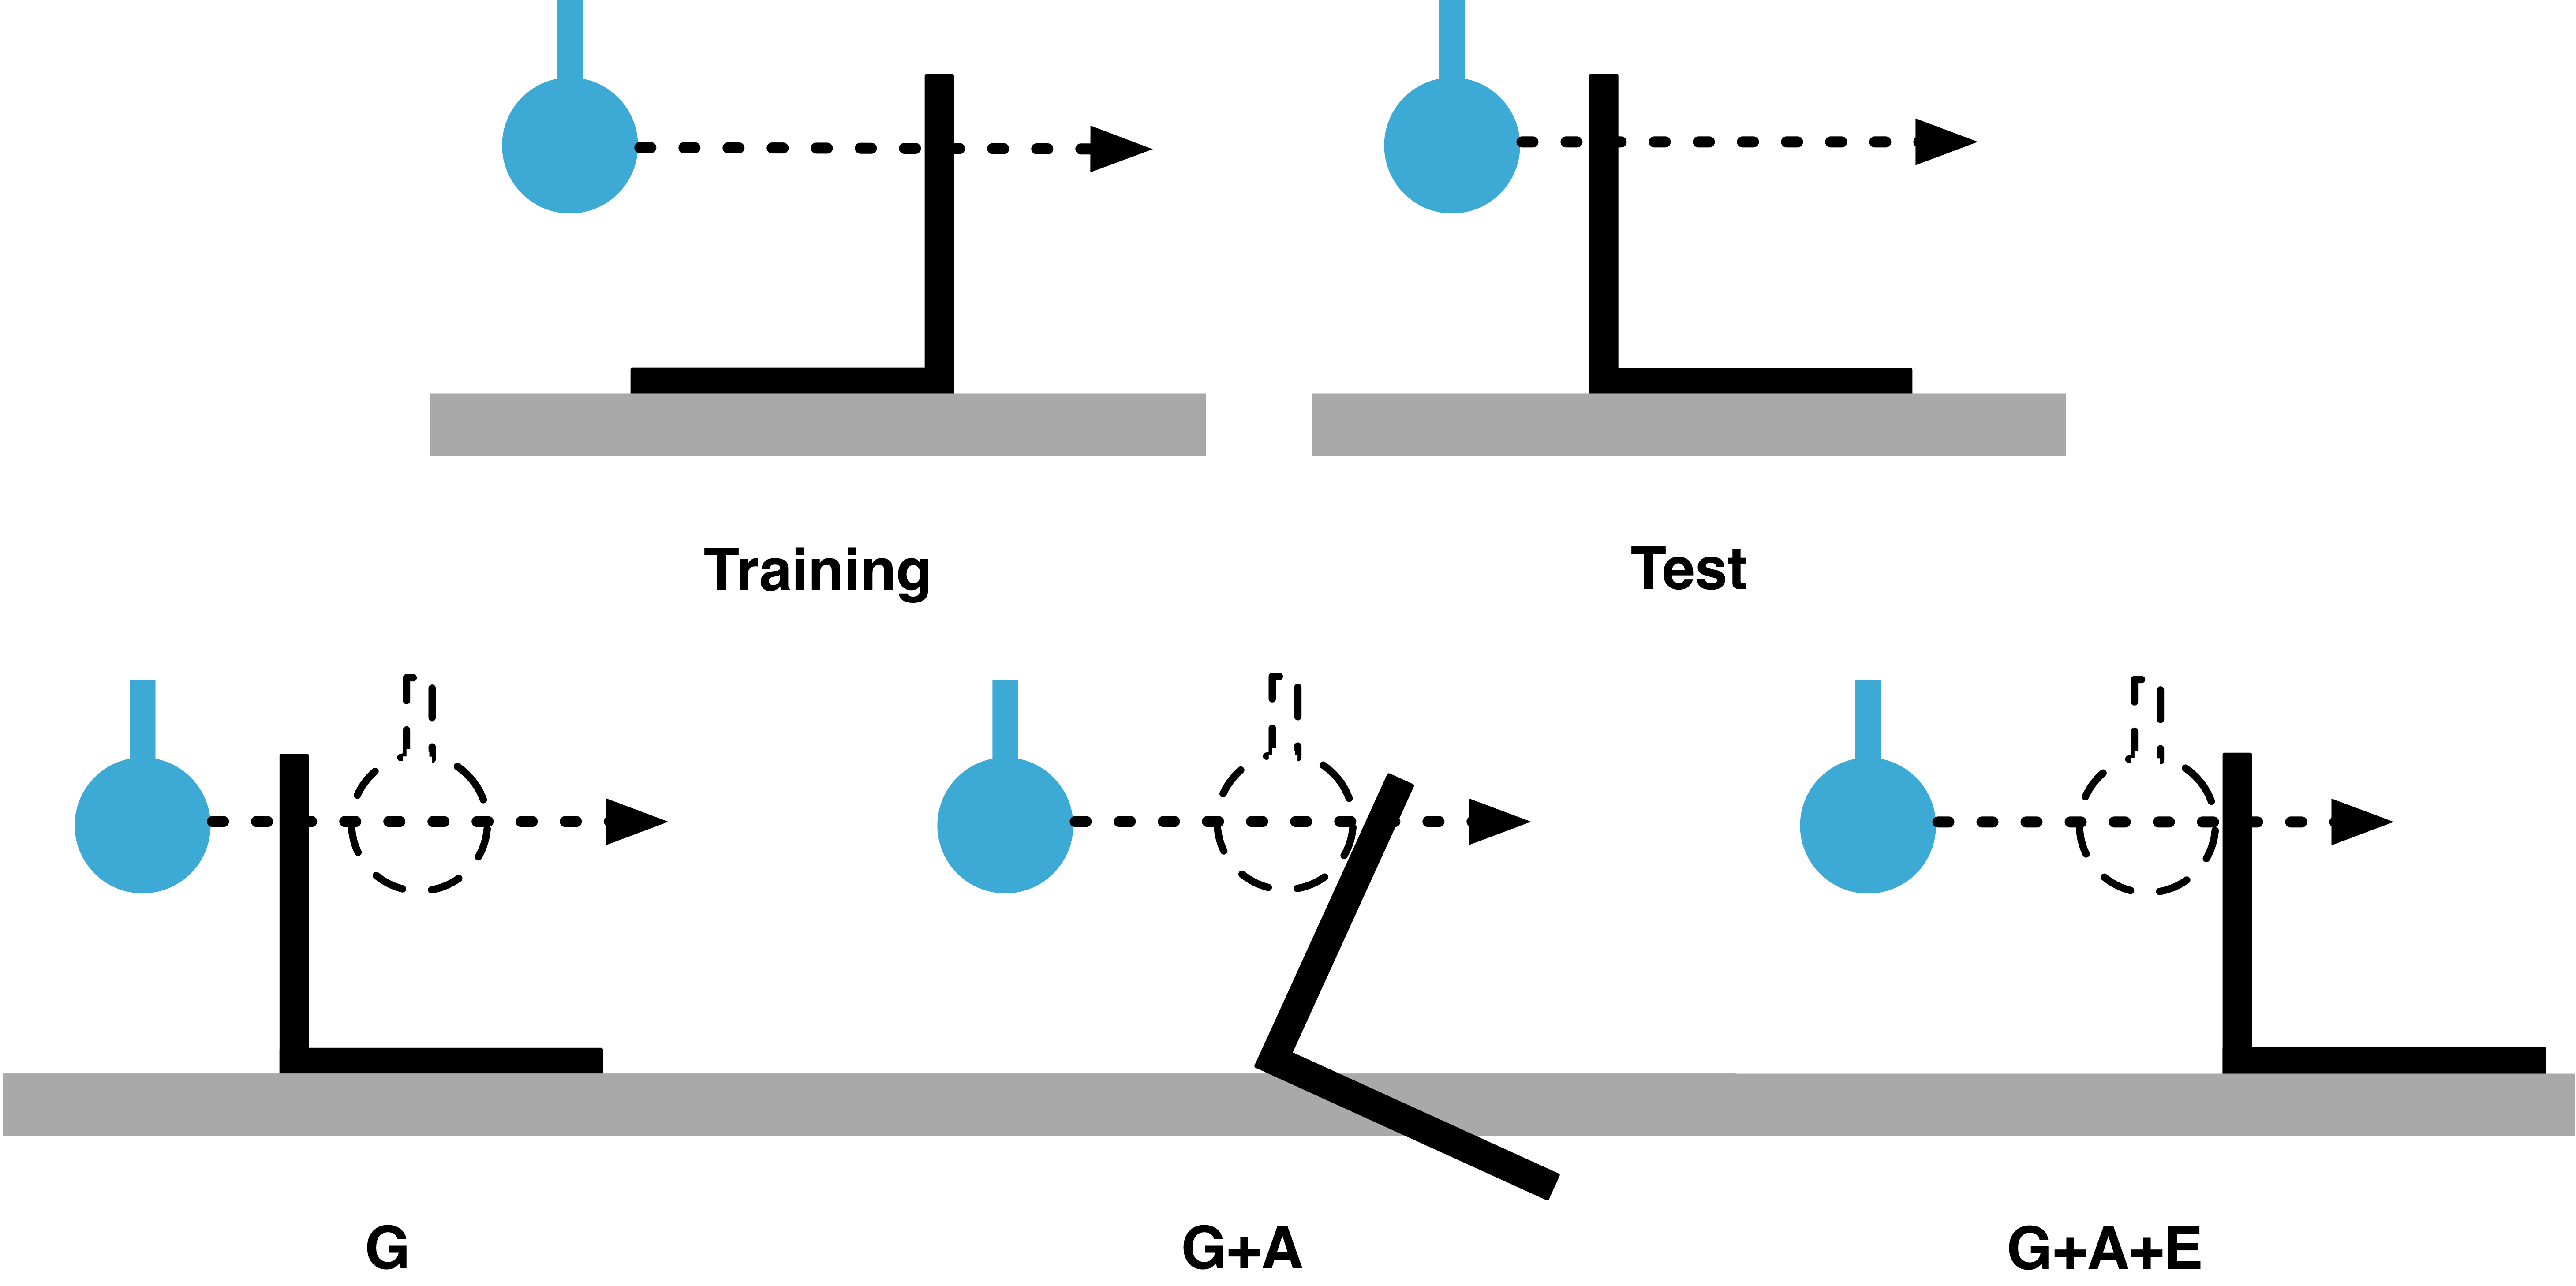
\includegraphics[width=\columnwidth]{BackPushToyExample}}
\caption[ToyExample]{Information for Action Transfer: an L-shaped object is pushed by a finger. Various predictors are trained solely on forward pushes (top left), but tested on backwards pushes (top right). The top panels show a training and a test push, whereas the bottom panels show predictions given different information (G, G+A and G+A+E) for the test push.}
\label{fig:ToyExample}
\end{figure}
One point is critical here: the above analysis only concerns what the information allows, it depends on the ability of the learner to
utilise it.  To test this we must incorporate the information into each learning framework. We can simply extend the regression and density
estimation frameworks to achieve this. For regression one way to incorporate the extra information $A^{L}_{t}$,$B^{L}_{t}$ and
$E^{Sk}_t$\hspace{-6pt}, $B^{Sk}_t$, provided by the agent and environment contacts, is simply to enlarge the domain of function~$f$
in Equation~\eqref{eq:Learning.short}, that is:
\begin{multline}
f'_{qs}: T^{A_t, B_t}, T^{B_t, O}, T^{A_{t}, A_{t+1}}, T^{A^{L}_t, B^{L}_t} \\ \{, T^{E^{Sk}_t,B^{Sk}_t}\}_{k=1 \ldots N} \longrightarrow T^{B_{t}, B_{t+1}}
\label{eq:Learning.augmented}
\end{multline}
\noindent Unfortunately, because the dimensionality of the domain of $f'_{qs}$ grows with the number of environment contacts $N$,
the difficulty of learning the mapping $f'_{qs}$ rapidly increases as environment contacts are added.

The conditional probability density (CPD) $p_{qs}$ over possible object motions $T^{B_{t}, B_{t+1}}$~\citep{kopicki_prediction_2009} is augmented as follows:
\begin{multline}
p_{qs}(T^{B_{t}, B_{t+1}} | T^{A_t, B_t}, T^{B_t, O}, T^{A_{t}, A_{t+1}}, T^{A^{L}_t, B^{L}_t} \\ \{, T^{E^{Sk}_t,B^{Sk}_t}\}_{k=1 \ldots N})
\label{eq:Learning.density}
\end{multline}

Again the dimensionality of the conditioning variables makes density estimation hard as the number of contacts grows. One way around this in the density estimation case is to factorize the density in a way that reflects the contact structure. We consider this in the next section. 